\documentclass[a4paper,10pt]{report}
\usepackage[utf8]{inputenc}
\usepackage{graphicx}

\makeatletter 
  \DeclareRobustCommand*\textsubscript[1]{% 
    \@textsubscript{\selectfont#1}} 
  \newcommand{\@textsubscript}[1]{% 
    {\m@th\ensuremath{_{\mbox{\fontsize\sf@size\z@#1}}}}} 
\makeatother 


% Title Page
\title{\textbf{OPTICAL COMMUNICATION COMPONENTS \\ Lab 2}}
\author{Nicola Simoni, Tadewos Somano}
\date{University of Brescia, Faculty of Engineering\\A.Y. 2013-2014}


\begin{document}
\maketitle

\section*{Exercise 1}
To compute the attenuation coefficient $\alpha$ we use the ``cut-back'' method, cutting the fiber at various lengths and measuring 
the relative power. We compute the attenuation coefficient as: $$\alpha=\frac{P_2-P_1}{|L_2-L_1|}$$
Where $P_2 > P_1$.
In the following table are reported three measures:

\begin{center}
\begin{tabular}{l | c | r}
  \hline
  P\textsubscript{out} [dBm]& Length [m]& $\alpha$ [dB/m]\\
  \hline
  2.81 & 1 $\cdot 10^3$ & 2 $\cdot 10^{-4}$\\
  2.61 & 2 $\cdot 10^3$ & 2 $\cdot 10^{-4}$\\
  2.41 & 3 $\cdot 10^3$ & 2 $\cdot 10^{-4}$\\
  \hline  
\end{tabular}
\end{center}

The value stored in the module fiber is $2\cdot 10^{-4}$ [dB/m], so the computation of the attenuation coefficient works well.
\section*{Question 1}
In a real setup this couldn't work because we have launch losses that are unknown.
In the simulation, instead, we assume that all the power of the laser is transmitted into the fiber.


\section*{Question 2}
The difference between the two cases is the inversion of the chirp sign.
In Figure \ref{negdisp} is shown the waveform and the corresponding chirp function
that travels in the fiber with negative dispersion. In Figure \ref{posdisp} is shown the same signal that travels in a positive dispersion fiber.
It is easy to see that the second chirp function is equal to the first one, but with the sign inverted.

\begin{figure}[!ht]
  \centering
  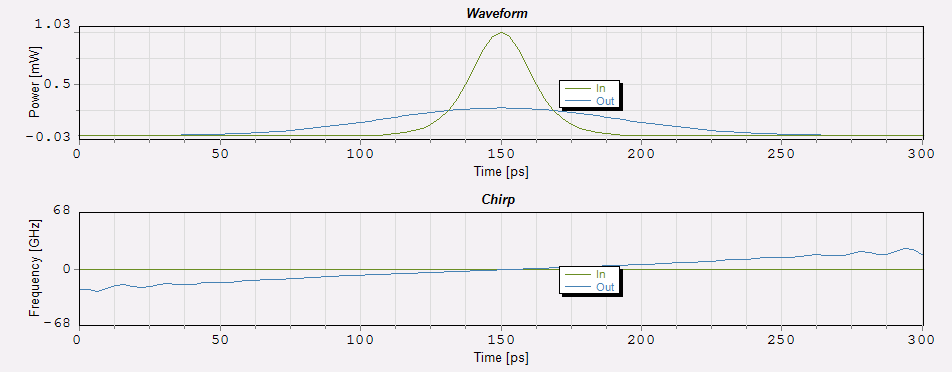
\includegraphics[width=12cm]{50km_neg_SignalAnalyzer_vtms1.png}\\
  \caption{Negative dispersion.}
  \label{negdisp}
\end{figure}

\begin{figure}[!ht]
  \centering
  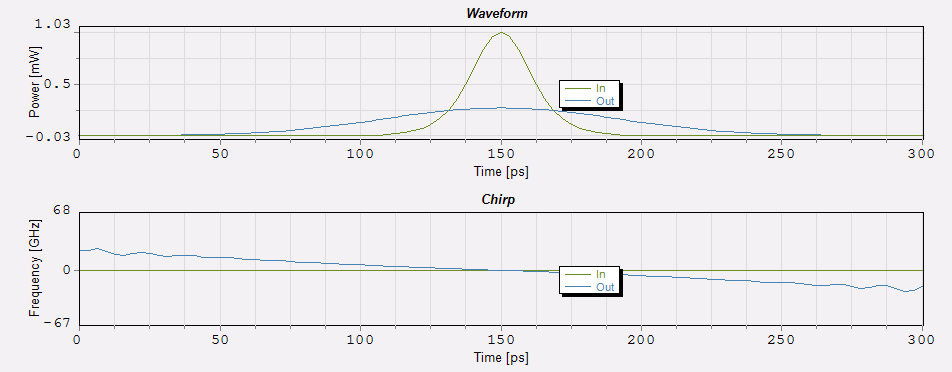
\includegraphics[width=12cm]{50km_SignalAnalyzer_vtms1.png}\\
  \caption{Positive dispersion.}
  \label{posdisp}
\end{figure}

% In Figure \ref{oneoptical} is shown the output spectrum of the signal.
% \begin{figure}[!ht]
%   \centering
%   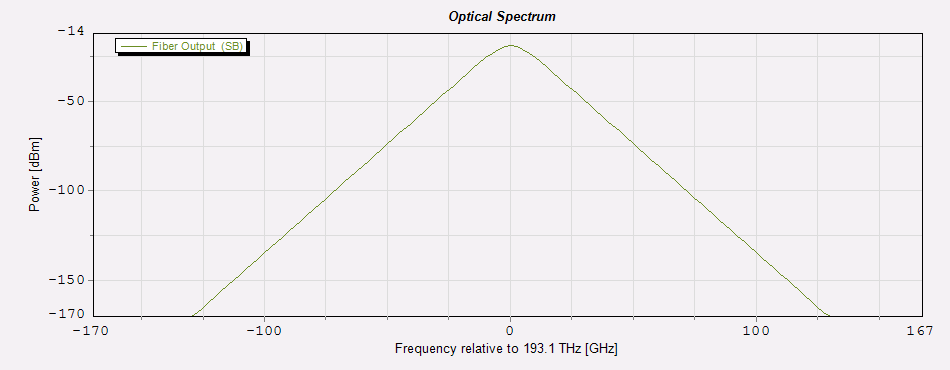
\includegraphics[width=12cm]{50km_spectrum.png}\\
%   \caption{Output spectrum.}
%   \label{oneoptical}
% \end{figure}

\newpage
\section*{Question 2.a}
In Figure \ref{twopuls} is shown the case of two transmitted pulses, separated by a time of 100 ps.
The green function represents the signal at the input of the fiber. As we can see it has no chirp.
The blue function, instead, represents the signal at the output of the fiber, that is 50 Km long.
The dispersion value is equal to $1.6 \cdot 10^{-5} \ [s/m^2]$.
We can notice that the received signal is very different from the transmitted one: it is made of three pulses, where the central
one has the highest power. Moreover, the signal is chirped.
This happens because of dispersion phenomenon: while travelling, different spectral components of the pulses propagate with different velocities.
This causes the widening of the two pulses that interfere one with each other, causing a constructive sum that form the central pulse.

\begin{figure}[!ht]
  \centering
  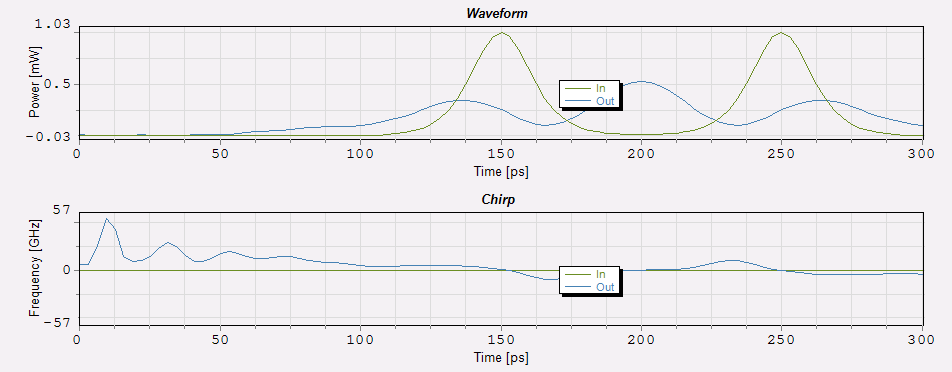
\includegraphics[width=12cm]{one_50km_SignalAnalyzer_vtms1.png}\\
  \caption{Propagation of two pulses.}
  \label{twopuls}
\end{figure}

% The optical power spectrum at the output is shown in Figure \ref{twooptical}.
% 
% \begin{figure}[!ht]
%   \centering
%   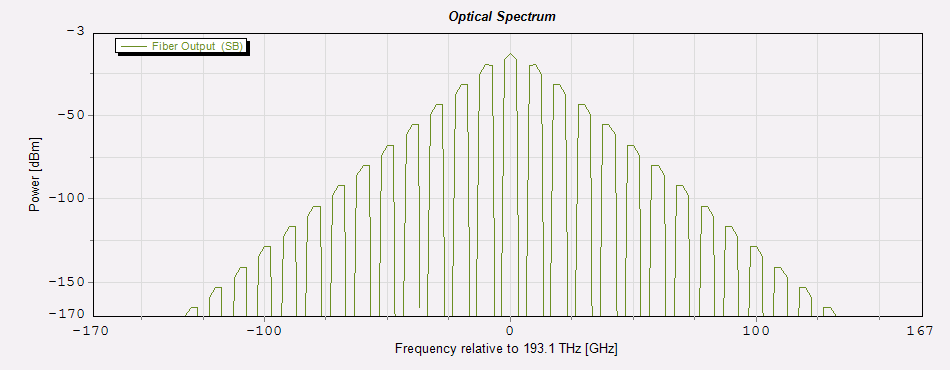
\includegraphics[width=12cm]{one_50km_spectrum.png}\\
%   \caption{Two pulses spectrum.}
%   \label{twooptical}
% \end{figure}


\newpage
\section*{Exercise 2}

In Figure \ref{berplot} are shown three plots of the BER versus the fiber length at three different bitrates: 2.5 Gbit/s (red dots),
5 Gbit/s (blue dots) and 10 Gbit/s (green dots). The distance varies from 80 Km to 140 Km with steps of 10 Km.

\begin{figure}[!ht]
  \centering
  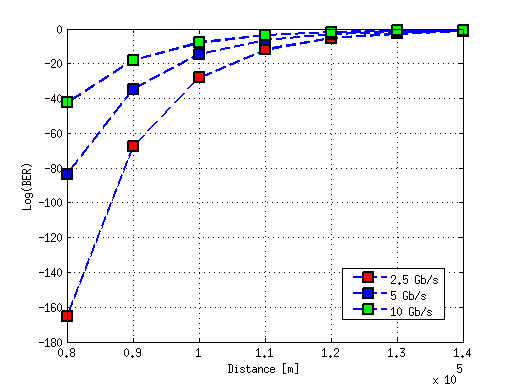
\includegraphics[width=12cm]{berplot.png}\\
  \caption{BER plots for 2.5 Gbit/s, 5 Gbit/s and 10 Gbit/s.}
  \label{berplot}
\end{figure}

In order to understand for which values of length we have acceptable BERs, 
we zoom the graph as shown in Figure \ref{berplotzoom}.

\begin{figure}[!ht]
  \centering
  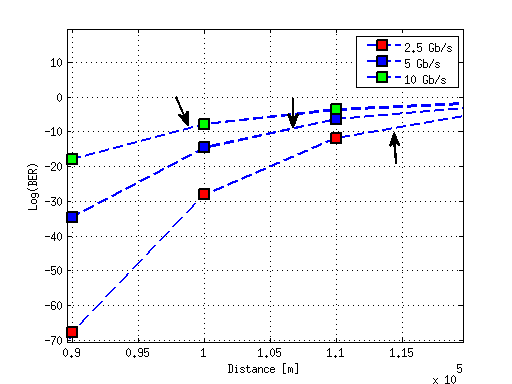
\includegraphics[width=12cm]{berplotzoom.png}\\
  \caption{Distance limits.}
  \label{berplotzoom}
\end{figure}

The maximum distances achievable are approximatively:
\begin{itemize}
 \item 2.5 Gbit/s $\longrightarrow$ $L=114500$ m
 \item 5 Gbit/s $\longrightarrow$ $L=106000$ m
 \item 10 Gbit/s $\longrightarrow$ $L=98800$ m
\end{itemize}

\section*{Exercise 3}
We fix the rate at 10 Gbit/s, sensitivity of receiver to $1.05 \cdot 10^{-5}\ W$ and average output power of the transmitter to $10^{-3}\ W$.
Dispersion value is set equal to the one of the previous exercise.
To compute the maximum distances for various attenuation coefficients we first convert the powers in dB:
$$P_{out}=10Log \Bigl(\frac{10^{-3}}{10^{-3}}\Bigr)=0 \ dBm$$
$$P_{rx}=10Log \Bigl(\frac{1.05 \cdot 10^{-5}}{10^{-3}}\Bigr)=-19.79 \ dBm$$

To compute the maximum lengths we use the equation: $$L_i=\frac{P_{out}-P_{rx}}{\alpha_i}$$
We obtain the following values:
\begin{itemize}
 \item $\alpha_1=0.4$ dB/Km $\longrightarrow$ $L_1 = 49.47$ Km
 \item $\alpha_2=0.6$ dB/Km $\longrightarrow$ $L_1 = 32.98$ Km
 \item $\alpha_3=0.8$ dB/Km $\longrightarrow$ $L_1 = 24.74$ Km
 \item $\alpha_4=1$ dB/Km $\longrightarrow$ $L_1 = 19.79$ Km
\end{itemize}


\section*{Exercise 4}
In Figure \ref{ber4} are shown the BERs over the distance with no attenuation, a dispersion of $1.6 \cdot 10^{-5} \ [s/m^2]$,
a dispersion slope of $80 \ [s/m^3]$ and zero non linear index.
The fiber length varies from 100 Km to 1400 Km with steps of 100 Km.

\begin{figure}[!ht]
  \centering
  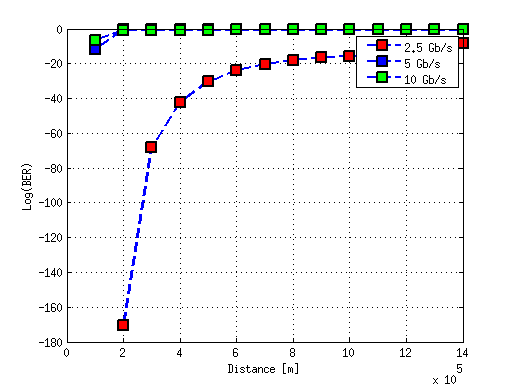
\includegraphics[width=12cm]{ber_es4.png}\\
  \caption{BER plots for 2.5 Gbit/s, 5 Gbit/s and 10 Gbit/s.}
  \label{ber4}
\end{figure}

We can observe that, for the bit rate of 2.5 Gbit/s, we can reach almost the whole length of the fiber within an acceptable BER, while
with the 5 Gbit/s rate we can travel for 20 Km from the starting point (100 Km) and with the 10 Gbit/s rate the BER is too high
even at the starting point.

In Figure \ref{eye1}, \ref{eye2} and \ref{eye3} are shown the eye diagrams at the distances: 1400 Km for the rates 2.5, 5 and 10 Gbit/s.

\begin{figure}
  \centering
  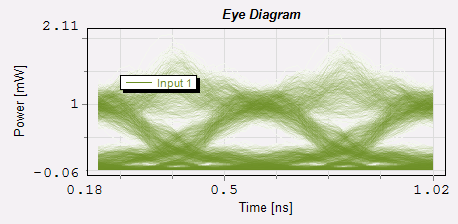
\includegraphics[width=10cm]{eye140km_2-5Gb.png}\\
  \caption{Eye diagram for 2.5 Gbit/s.}
  \label{eye1}
\end{figure}

\begin{figure}
  \centering
  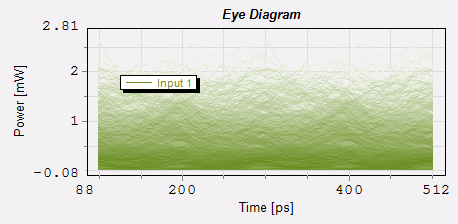
\includegraphics[width=10cm]{eye140km_5Gb.png}\\
  \caption{Eye diagram for 5 Gbit/s.}
  \label{eye2}
\end{figure}

\begin{figure}
  \centering
  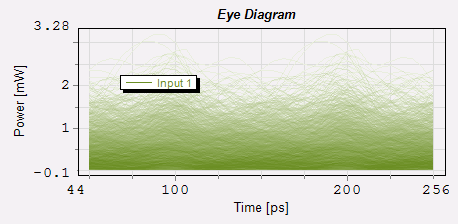
\includegraphics[width=10cm]{eye140km_10Gb.png}\\
  \caption{Eye diagram for 10 Gbit/s.}
  \label{eye3}
\end{figure}

The only acceptable is the one corresponding to a rate of 2.5 Gbit/s.


\section*{Question 3}
In Figure \ref{q3_1}, \ref{q3_2} and \ref{q3_3} are shown the plots of BER versus distance.
We use a loop in the fiber, in order to obtain faster plots. The fiber lengths are
respectively $10^5$, $10^5$ and $10^4$ meters. The other parameters are the same of the ones used in Exercise 4.
The intersection points have been read on the zoom of the graphs in the point corresponding at a BER of $10^{-9}$,
multiplying these points with the fiber lengths we obtained the maximum distances reachable:
\begin{itemize}
 \item 2.5 Gbit/s $\longrightarrow$ $L=1270000$ Km
 \item 5 Gbit/s $\longrightarrow$ $L=269800$ Km
 \item 10 Gbit/s $\longrightarrow$ $L=81260$ Km
\end{itemize}


\begin{figure}[!ht]
  \centering
  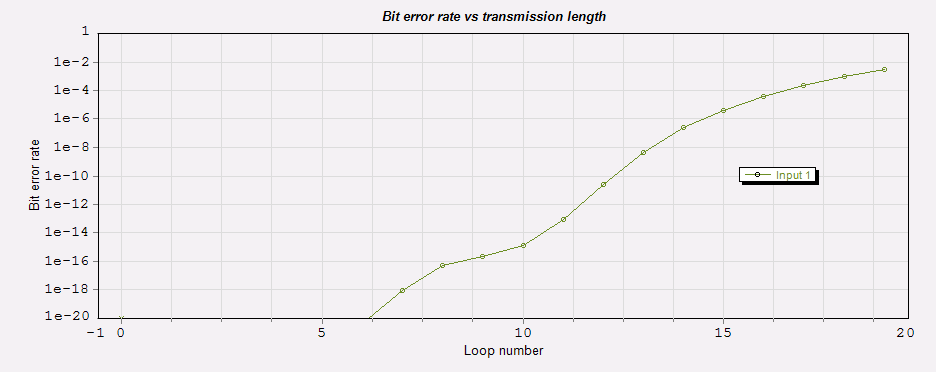
\includegraphics[width=12cm]{q3_2-5gb.png}\\
  \caption{BER plot at 2.5 Gbit/s.}
  \label{q3_1}
\end{figure}

\begin{figure}[!ht]
  \centering
  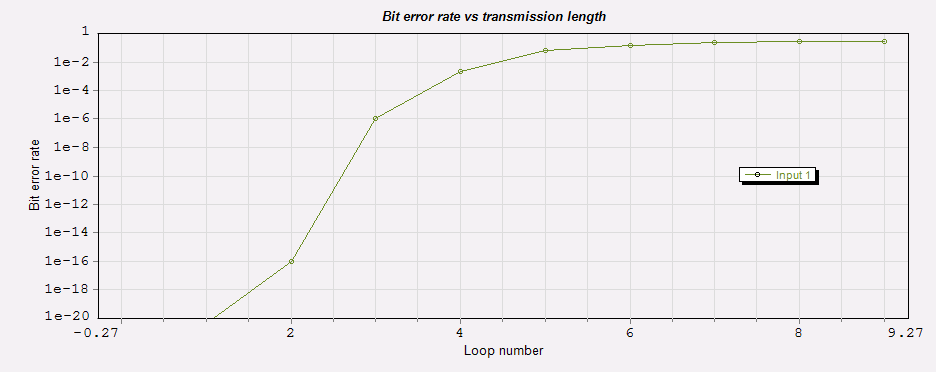
\includegraphics[width=12cm]{q3_5gb.png}\\
  \caption{BER plot at 5 Gbit/s.}
  \label{q3_2}
\end{figure}

\begin{figure}[!ht]
  \centering
  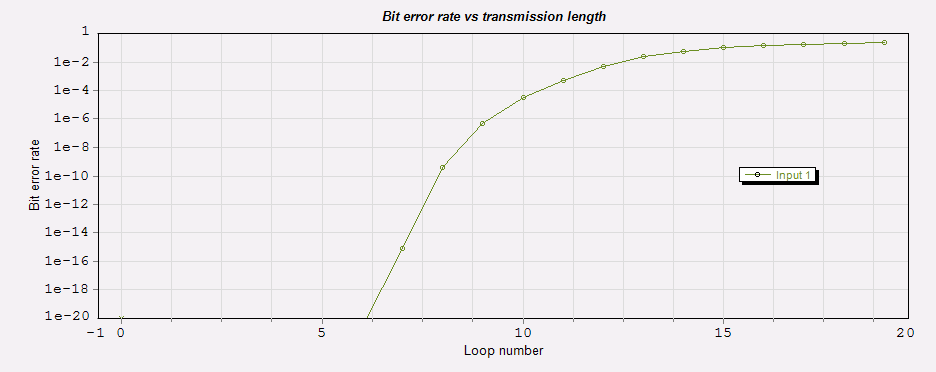
\includegraphics[width=12cm]{q3_10gb.png}\\
  \caption{BER plot at 10 Gbit/s.}
  \label{q3_3}
\end{figure}


\newpage
\section*{Exercise 5}
We fix the bit rate at 10 Gbit/s and we plot the BER versus the following values of dispersion:
\begin{itemize}
 \item $D_1=10^{-5} \ [s/m^2]$
 \item $D_2=4\cdot 10^{-6} \ [s/m^2]$
 \item $D_3=2\cdot 10^{-6} \ [s/m^2]$
 \item $D_4=10^{-6} \ [s/m^2]$
\end{itemize}


In Figure \ref{5_1}, \ref{5_2}, \ref{5_3} and \ref{5_4} are shown the plots.
The values of the fiber spans are respectively: $10^4$, $10^5$, $10^5$ and $5\cdot 10^5$ meters.

\begin{figure}[!ht]
  \centering
  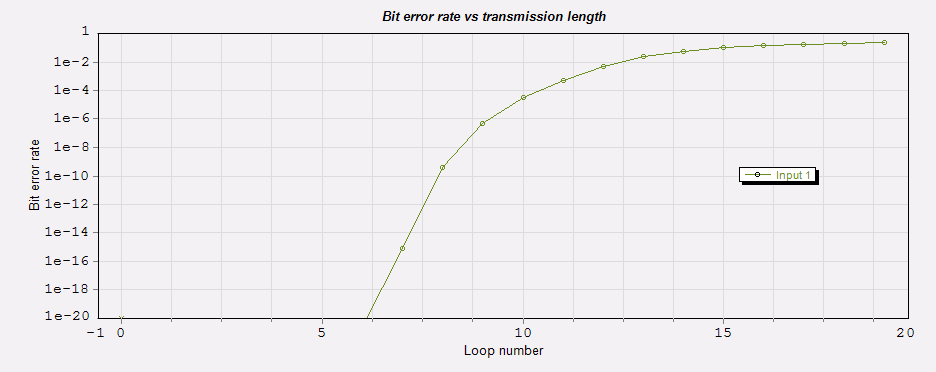
\includegraphics[width=12cm]{es5_1.png}\\
  \caption{BER plot with dispersion $D_1$.}
  \label{5_1}
\end{figure}

\begin{figure}[!ht]
  \centering
  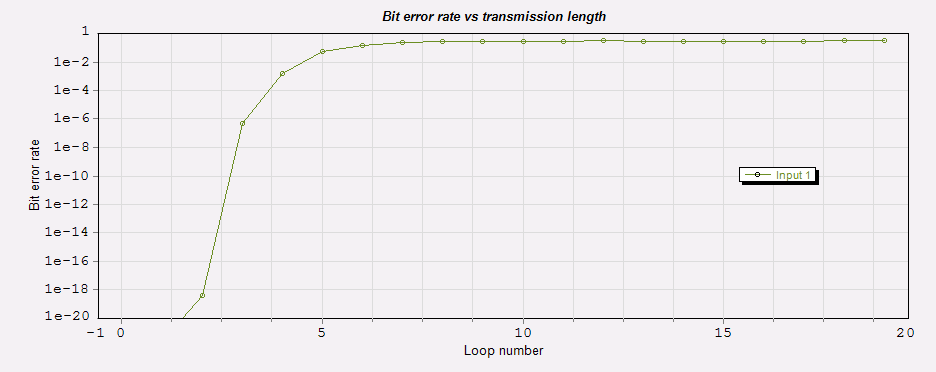
\includegraphics[width=12cm]{es5_2.png}\\
  \caption{BER plot with dispersion $D_2$.}
  \label{5_2}
\end{figure}

\begin{figure}[!ht]
  \centering
  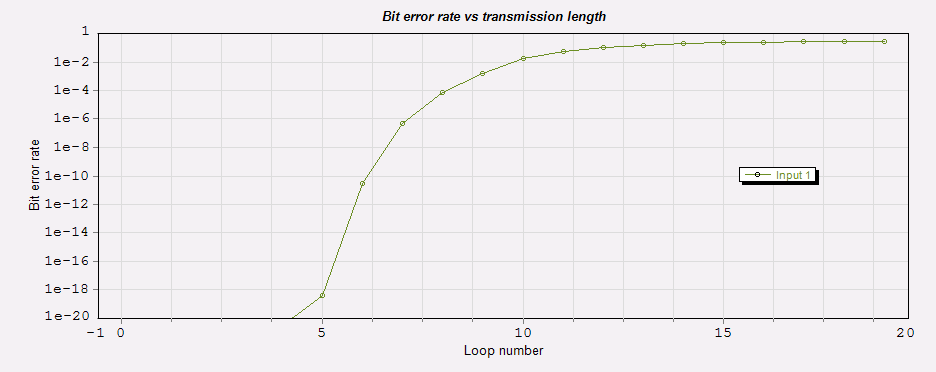
\includegraphics[width=12cm]{es5_3.png}\\
  \caption{BER plot with dispersion $D_3$.}
  \label{5_3}
\end{figure}

\begin{figure}[!ht]
  \centering
  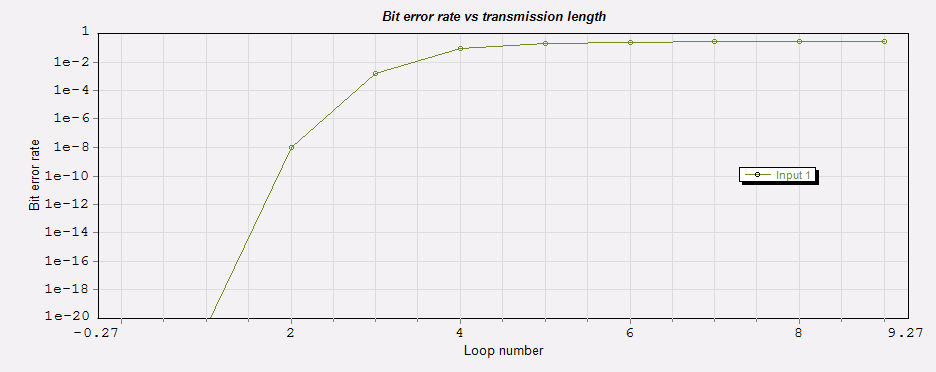
\includegraphics[width=12cm]{es5_4.png}\\
  \caption{BER plot with dispersion $D_4$.}
  \label{5_4}
\end{figure}


\newpage
\section*{Exercise 6}
In Figure \ref{plotes6} is are shown the BERs versus distance for the bit rates 2.5, 5 and 10 Gbit/s.
The length of the fiber varies from 80 Km to 130 Km in steps of 10 Km.
The attenuation is set to $2 \cdot 10^{-4} \ [dB/m]$, dispersion to $1.6 \cdot 10^{-5}\ [s/m^2]$,
dispersion slope to $80 \ [s/m^3]$ and non linear index to zero.

\begin{figure}[!ht]
  \centering
  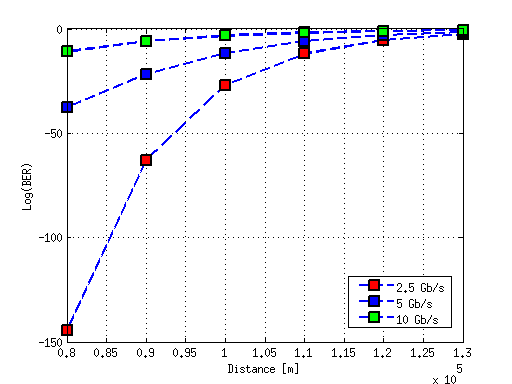
\includegraphics[width=12cm]{es6.png}\\
  \caption{BER plots for 2.5 Gbit/s, 5 Gbit/s and 10 Gbit/s.}
  \label{plotes6}
\end{figure}

\section*{Exercise 7}
Comparing the results with the ones in the Exercise 3 (in which we considered only attenuation), we can
conclude that, for the 10 Gbit/s signal, is the dispersion that determines the maximum transmission distance, while for the
2.5 Gbit/s is the attenuation.
To find the maximum distances for a ber less or equal than $10^{-9}$, we zoom the plot of Figure \ref{plotes6}, and we obtain
the following values:
\begin{itemize}
 \item 2.5 Gbit/s $\longrightarrow$ 96700 m
 \item 5 Gbit/s $\longrightarrow$ 86300 m
 \item 10 Gbit/s $\longrightarrow$ 64420 m
\end{itemize}




\section*{Exercise 8}
We fix the bit rate to 5 Gbit/s and we plot the BER versus distance for the following values of dispersion:
\begin{itemize}
 \item $D_1=10^{-5} \ [s/m^2]$
 \item $D_2=4\cdot 10^{-6} \ [s/m^2]$
 \item $D_3=2\cdot 10^{-6} \ [s/m^2]$
 \item $D_4=10^{-6} \ [s/m^2]$
\end{itemize}

In the Figures \ref{8_1}, \ref{8_2}, \ref{8_3} and \ref{8_4} are shown the relative plots.
The computed maximum length values are:
\begin{itemize}
 \item $L_1 = 88470 \ m$
 \item $L_2 = 89490 \ m$
 \item $L_3 = 89530 \ m$
 \item $L_4 = 89470 \ m$
\end{itemize}

Smaller the dispersion more is the distance that can be reached.

\begin{figure}[!ht]
  \centering
  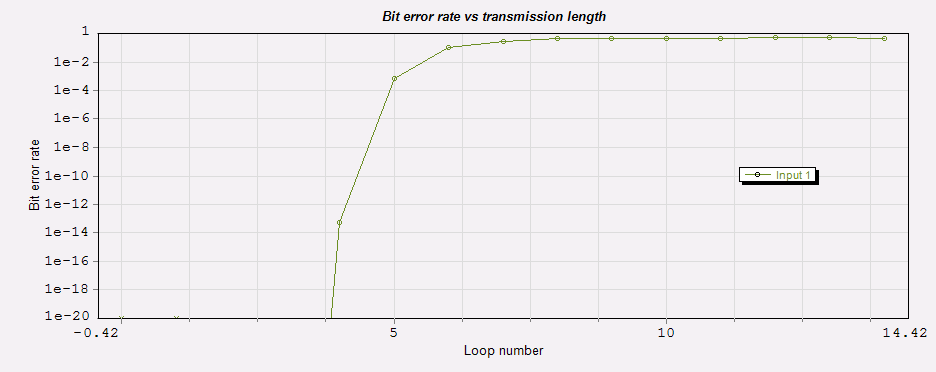
\includegraphics[width=12cm]{es8_1.png}\\
  \caption{BER plot with dispersion $D_1$.}
  \label{8_1}
\end{figure}

\begin{figure}[!ht]
  \centering
  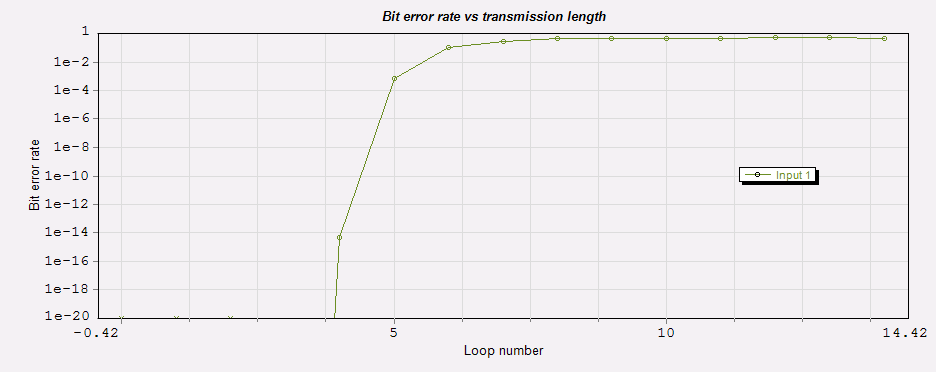
\includegraphics[width=12cm]{es8_2.png}\\
  \caption{BER plot with dispersion $D_2$.}
  \label{8_2}
\end{figure}

\begin{figure}[!ht]
  \centering
  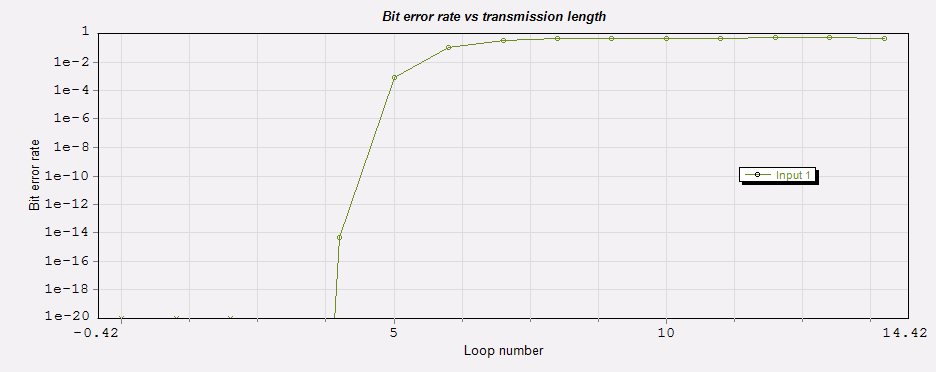
\includegraphics[width=12cm]{es8_3.png}\\
  \caption{BER plot with dispersion $D_3$.}
  \label{8_3}
\end{figure}

\begin{figure}[!ht]
  \centering
  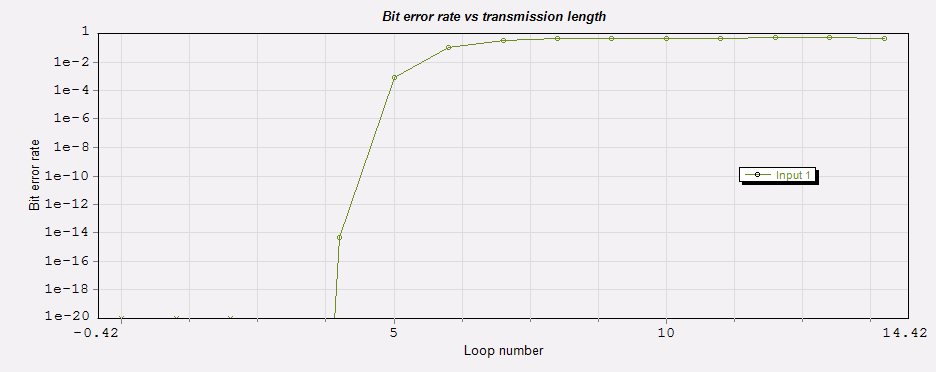
\includegraphics[width=12cm]{es8_4.png}\\
  \caption{BER plot with dispersion $D_4$.}
  \label{8_4}
\end{figure}



\newpage
\section*{Exercise 9}
We consider a case in which we have the following parameters: attenuation $2 \cdot 10^{-4} \ [dB/m]$, dispersion $1.6 \cdot 10^{-5}\ [s/m^2]$,
dispersion slope $80 \ [s/m^3]$, non linear index $2.6 \cdot 10^{-2}\ [m^2/W]$. The fiber length is fixed to $10^5 \ m$ and we increase the
transmission power from 0 dBm up to 20 dBm with steps of 4 dB.\\
In Figure \ref{es9} are shown the plots of BER versus power, for 2.5, 5 and 10 Gbit/s rates.

\begin{figure}[!ht]
  \centering
  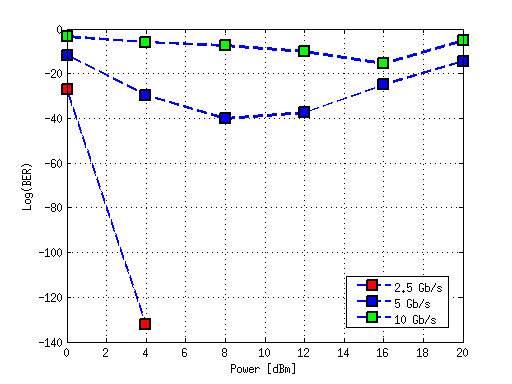
\includegraphics[width=12cm]{es9.png}\\
  \caption{BER plots for 2.5 Gbit/s, 5 Gbit/s and 10 Gbit/s.}
  \label{es9}
\end{figure}

At this fiber length the only rate which BER is not always acceptable (it is higher than $10^{-9}$) is the 10 Gbit/s one.
It is good starting from a power of 10.2 dBm, it decreases but then increases again when the power is more than 16 dBm.
The 5 Gbit/s BER is always acceptable: it decreases until a power of 8 dBm and then increases, while the 10 Gbit/s BER always decreases.
Non linearities increase with the increasing of the bit rate.






\end{document}